\chapter{Results}
\label{sec:results}
In previous chapters, there were introduced different methods available for selected use cases in research in biology and medicine. 
%\section{Virtual Infrastructure}
%\label{sec:resultsinfrastructure}
As each of the use cases and available system was proposed on different operating system platform, different architecture and or different middleware the virtualization was utilized to build the virtual infrastructures for purposes of each project. The paper \cite{kulhanek2010c} \emph{Infrastructure for Data Storage and Computation in Biomedical Research} in Appendix~\ref{app:infrastructure} describes result of establishing the virtualization on physical infrastructure to share computational power among different platforms.

\section{Medical Images}
\label{sec:resultsimages}

%Within the virtual infrastructure, the pilot grid infrastructure was established in the location of First Faculty of Medicine, Charles University in Prague, Central Military Hospital in Prague and CESNET association. And the Globus Toolkit middleware and Globus MEDICUS implementation was installed on linux based virtual machines using XEN hypervisor providing pilot services to access this grid based PACS system.

The pilot infrastructure of several servers were installed in several institutions in Prague, Czech Republic and Globus Toolkit and Globus MEDICUS was installed on them. The paper \cite{kulhanek2009}  \emph{Processing of Medical Images in Virtual Distributed Environment} in Appendix~\ref{app:processing} published details about the integration of Globus MEDICUS instance with MeDiMed project with conclusion that such integration via DICOM protocol is almost seamless and may bring high benefits for researcher if such grid-based system is joined with a production system for exchanging clinical DICOM data. 

\section{Remote access to voice analysis}
\label{sec:resultsvoice}

The paper \cite{kulhanek2010b} \emph{Remote Analysis of Human Voice--Lossless Sound Recording Redirection} in the Appendix~\ref{app:remote} published technical details and results of customizing RDP protocol for lossless sound recording redirection and remote access via remote desktop feature of Windows platform to the application to analyze human voice and produce voice range profile for further use. 

Additionally, the custom RDP plugin with the ParVRP and RealVoiceLab software to redirect the sound recording without loss of information was packaged as a virtual machine template and  deployed in the pilot virtual infrastructure next to the test instance of Globus MEDICUS. The virtual machine template was also deployed to different cloud computing infrastructures. One to the Amazon EC2\footnote{\url{http://aws.amazon.com/ec2/} accessed February 2015} and second to the pilot scientific cloud launched in the begining of 2012 --MetaCloud\footnote{\url{http://www.metacentrum.cz/en/cloud/} accessed February 2015}. Such comparison was presented to the user and technical community within CESNET and EGI organization in EGI Technical Forum 2012\cite{Kulhanek2012a}.

\section{Parameter Estimation}
\label{sec:resultsestimation}

The paper \cite{Kulhanek2014Parameters} \emph{Parameter estimation of complex mathematical models of human physiology using remote simulation distributed in scientific cloud} in Appendix~\ref{app:parameter} published the architecture and measurement of speedup achieved on estimating parameters of three  different types of models from the non-complex, medium-complex and complex model with conclusion that only medium-complex and complex model may benefit from the architecture as the communication overhead may become major for simple models and decrease overall performance. 

Additionally, scientific result was published in the paper \cite{Matejak2014sj} \emph{Adair-Based Hemoglobin Equilibrium with Oxygen, Carbon Dioxide and Hydrogen Ion Activity} in Appendix~\ref{app:adair} where a mathematical model of hemoglobin integrating \ce{O_2}, \ce{CO_2} and \ce{H^+} binding based on theoretical principles, which were verified on the parameter estimation algorithm system\cite{Kulhanek2014Parameters} together with methods available in Wolfram \emph{MATHEMATICA} 9.0\footnote{\url{http://www.wolfram.com/mathematica/}accessed February 2015}.

Thus overall performance and speedup estimation were tested against the Modelica implementation of complex physiological model HumMod \cite{Kofranek2011hummod}, the Modelica implementation of model of haemodynamics of cardivaoscular system presented by Meurs \cite{Meurs2011}, the model of binding gases to hemoglobin named as Matejak2014 \cite{Matejak2014sj} and trivial model of a curve $f(x)$ with 4 parameters $a,b,c,d$ defined as $ f(x)=a\cdot sin(b\cdot (x-c))+x\cdot d$ and named as "SinusCurve".
\sisetup{round-mode=figures,round-precision = 4}
\begin{table}[htb]
\footnotesize
\begin{tabular}{|l|r|r|r|r|r|r|r|}
\hline
complexity & name & T1$_{[s]}$ & T2$_{[s]}$ & T3$_{[s]}$ & T4$_{[s]}$ & $\alpha$ & $S$ \\
\hline
high & HumMod \cite{Kofranek2011hummod} & $\num{4639}$ & $\num{4639}$ & $\num{4618}$ & $\num{4616}$ & $\num{8.85837717978788E-005}$ & $\num{11288.7493917249}$ \\
medium & Meurs2011\cite{Meurs2011} & $\num{661.817}$ & $\num{661.490}$ & $\num{634.694}$ & $\num{634.457}$ & $\num{0.0004940943}$ & $\num{2023.9051987766}$ \\
low & Matejak2014\cite{Matejak2014sj} & $\num{17.868}$ & $\num{17.610}$ & $\num{1.399}$ & $\num{1.123}$ & $\num{0.014439221}$ & $\num{69.2558139535}$ \\
trivial & SinusCurve & $0.073$ & $0.020$ & x & x &  $\num{0.7260273973}$ & $\num{1.3773584906}$\\
\hline
\end{tabular}
\caption{Time spent in different parts of the parameter estimation algorithm for 1 processor deployment. Genetic algorithm works with population of $120$ individuals for $10$ generations. T1 -- is the whole time of the computation, T2 -- is the time of the computation, which can be parallelized, T3 -- time spent within worker node, T4 -- time spent in simulation, $\alpha$ -- computed as $1-(T2/T1)$ and $S$ is theoretical speedup limit per Amdahl's law ($1/\alpha$) eq.(\ref{eq:amdahl}).}
\label{table:speedupresult}
\end{table}

\begin{table}[htb]
\footnotesize
\begin{tabular}{|l|r|r|r|r|r|r|r|}
\hline
complexity & name & T1$_{[s]}$ & T2$_{[s]}$ & T3$_{[s]}$ & T4$_{[s]}$ & $\alpha$ & $S$ \\
\hline
high & HumMod \cite{Kofranek2011hummod} & $\num{6463.217}$ & $\num{6460.937}$ & $\num{6451.079}$ & $\num{6458.253}$ & $\num{0.000352766}$ & $\num{2834.744}$ \\
medium & Meurs2011\cite{Meurs2011} & $\num{699.631}$ & $\num{699.228}$ & $\num{697.907}$ & $\num{696.948}$ & $\num{0.000576018}$ & $\num{1736.057072}$ \\
low & Matejak2014\cite{Matejak2014sj} & $\num{2.893}$ & $\num{2.373}$ & $\num{1.228}$ & $\num{1.149}$ & $\num{0.17974421}$ & $\num{5.563461538}$\\ \hline
\end{tabular}
\caption{Same as table \ref{table:speedupresult}, but measured on local cluster deployment with reduced communication overhead.}
\label{table:speedupresult2}
\end{table}

The computation time of single simulation depends on model complexity number of compared values. Based on the findings, the simulation of the models were divided into 4 groups depending on its demand to compute 1200 simulations. Fraction $\alpha$ and speedup limit per Amdahl's law was stated in Tables \ref{table:speedupresult} and \ref{table:speedupresult2}. 

Difference between $T2$ and $T3$ is an overhead introduced by the network communication between genetic algorithm and worker nodes deployed in cloud deployment provided by CESNET NGI department METACENTRUM\footnote{\url{http://www.metacentrum.cz} accessed March 2015}. The network overhead can be eliminated in serial implementation by directly integrating simulation into genetic algorithm, therefore, a hypothetical serial execution time estimated without the network overhead is considered and compared in Table \ref{table:overhead}.

\begin{table}[ht]
\footnotesize
\begin{tabular}{|l|r|r|r|r|r|r|r|r|}
\hline
& \multicolumn{4}{c|}{distributed in cloud} & \multicolumn{4}{c|}{distributed in local cluster} \\
 & \multicolumn{2}{c|}{overhead} & \multicolumn{2}{c|}{est. serial} & \multicolumn{2}{c|}{overhead} & \multicolumn{2}{c|}{est. serial} \\
model name & T2-T3$_{[s]}$ & fraction$_{[\%]}$ & $T_{es [s]}$ & $S_{es}$ & T2-T3$_{[s]}$ & fraction$_{[\%]}$ & $T_{es [s]}$ & $S_{es}$\\
\hline
HumMod \cite{Kofranek2011hummod} & $\num{20.983}$ & $\num{0.45225141}$ & $\num{4618.693}$ & $\num{1.0045430601}$ & $\num{9.858}$ & $\num{0.15252466}$ & $\num{6453.359}$ & $\num{1.0015275766}$ \\
Meurs2011 \cite{Meurs2011} & $\num{26.796}$ & $\num{4.04885338}$ & $\num{635.021}$ & $\num{1.0421970297}$ & $\num{1.321}$ &  $\num{0.18881382}$ & $\num{698.310}$ &$\num{1.00189171}$\\
Matejak2014\cite{Matejak2014sj} & $\num{16.211}$ & $\num{90.72643833}$ & $\num{1.657}$ & $\num{10.7833433917}$ & $\num{1.145}$ &  $\num{39.57829243}$ & $\num{1.748}$ &$\num{1.6550343249}$\\
\hline
\end{tabular}
\caption{ Comparison in cloud deployment vs. local cluster deployment of communication overhead, it's fraction in whole computation introduced by network transfer and latency. And estimated time and speedup if the worker will be replaced by serial version of computation without communication overhead: $T_{es}$ -- estimated time of serial version of computation. $S_{es}$ -- estimated speedup of serial version of computation against the parallel on 1 processor.}
\label{table:overhead}
\end{table}

The speedup was measured on 10 - 60 CPUs and compared to predicted speedup as seen in figure \ref{fig:amdahlres}). Different measurement was done using 80 and 160 CPUs with as seen in table \ref{table:speedupresult3}.

\begin{table}[htb]
\footnotesize
\begin{tabular}{|l|r|r|r|}
\hline
complexity & name & S(80)$_{[s]}$ & S(160)\\
\hline
high & HumMod \cite{Kofranek2011hummod} & $\num{85.2037411462}$ & $\num{161.8546206791}$ \\
medium & Meurs2011\cite{Meurs2011} & $\num{72.7343363629}$ & $\num{68.9392708333}$ \\
low & Matejak2014\cite{Matejak2014sj} & $\num{15.7039901564}$ & $\num{15.373}$\\ \hline
\end{tabular}
\caption{Scalability on 80 CPUs and 160 CPUs of genetic algorithm with population 640 individuals for 20 generations on different cluster, performed about 10 times more simulation. Speedup estimated based on the T1 column of table \ref{table:speedupresult}.}
\label{table:speedupresult3}
\end{table}

\begin{figure}[htb]
    \centering
    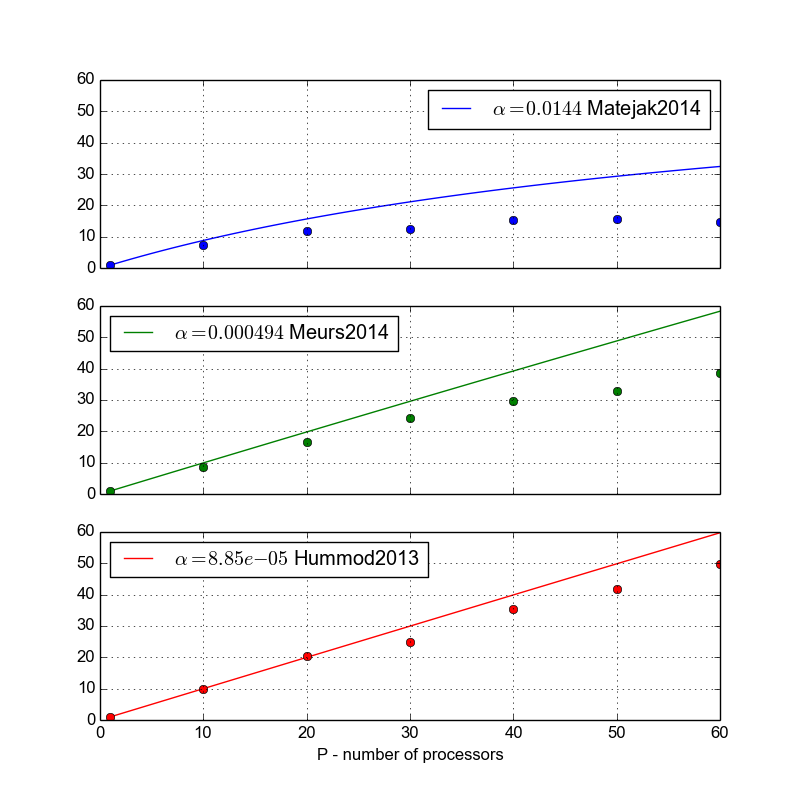
\includegraphics[width=0.9\textwidth]{chapter7/speedup.png}
    \caption{Estimated speedup (lines) per Amdahl's law (eq.\ref{eq:amdahl} \cite{Amdahl1967}) for different $\alpha$ of several Modelica models and real measured speedup (points) on cloud deployed on 1-6 virtual machines on physical hardware (2x 6-core Intel E5-2620 2GHz, 1Gbit/s Ethernet.)  }
    \label{fig:amdahlres}
\end{figure}

To summarize the results, the simple models scale up to the 20 processors with speedup of 15. Medium scales up to 80 processors with speedup about 72 and complex models scales up to 160 processors with speedup near 160. Practically there were obtained good approximation after 20 generation and good estimation after another 180 generations, which implicates that the computation time could be reduced from 5 days to 48 minutes in the case of HumMod and from 18 hours to 15 minutes in case of medium complex model.

The deployment on local cluster reduces the communication overhead, however is limited by available processors to compute concurrently, thus should be considered for the boundary cases like the simple models. The following statement could be made:
\begin{itemize}
\item{If the alpha fraction is major, then serial computation of parameter estimation algorithm without communication overhead will perform best. This is case of the trivial function. }
\item{If the alpha fraction is minor, but the network overhead is still major a computation on local cluster or virtual HPC cluster should be considered. This is the case of the low complex model simulation "Matejak2014"\cite{Matejak2014sj}.} 
\item{If the alpha fraction is minor and network overhead is also minor, then distributed computation e.g. in cloud-computing environment is worth to be used. This is case  of medium and high complex model simulation of "Meurs2011"\cite{Meurs2011} and "HumMod2013"\cite{Kofranek2011hummod}.}
\end{itemize}

\begin{figure}[htb]
    \centering
    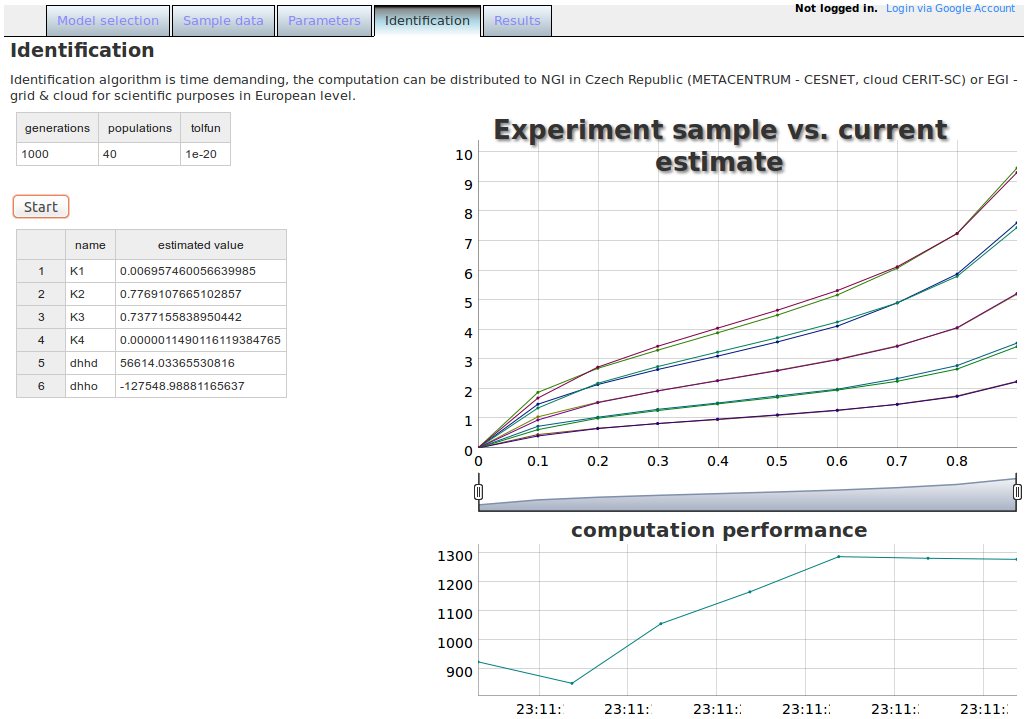
\includegraphics[width=1\textwidth]{chapter7/app-physiovalues.png}
    \caption{User interface of web application for parameter estimation. In this case for the model Matejak2014\cite{Matejak2014sj}. The top left table list the parameters for the genetic algorithm(1000 generations with population size of 40 and cumulative change in generation limit which ends the algorithm earlier). The middle left table shows model parameters and current best values which fits the sample data. Chart shows how the sample data fits with the model simulation. The right bottom chart shows the performance of computation in number of model simulations per second.}
    \label{fig:app.physiovalues}
\end{figure}

\subsection{Parameter Sweep}
\label{sec:resultsboinc}
The desktop grid BOINC system was established for parameter sweep application. The established project \emph{Physiome@home} and it's project web page \url{http://physiome.lf1.cuni.cz/ident3/physiome} manages workunits tasks which are sent to and executed by BOINC workers. The worker application is a packaged model exported as FMU for Windows platform and wrapper application which communicates with BOINC manager on the desired volunteer computer. 

%This project is now  distribute computational tasks into computers in scholar labs, which may in iddle time contribute to the computing demands. Because BOINC is very popular and users joins to a teams to compete with several types of competition, this particular project attracts after 2 weeks 78 participants from all around the world. 

%\section{Summary}
%
%A pilot repository of physiological model values was established at the web domain \url{http://www.physiovalues.org}. It contains links to the described web based application as well as an web application for web-based simulation and visualisation. 

\subsection{Remote Simulation and Local Visualization}
As an extra result of an architecture for parameter estimation is a hybrid web simulator system, where single instance of a worker node is utilized as a backend for simulation engine. Frontend presented as a web application implemented using HTML and Javascript language visualizes the simulation values obtained from the worker node performing the simulation as seen in figure \ref{fig:sim.physiovalues}.
The results were published in \cite{Kulhanek2013c} and popularized in \cite{Kulhanek2013b}.
\begin{figure}[htb]
    \centering
    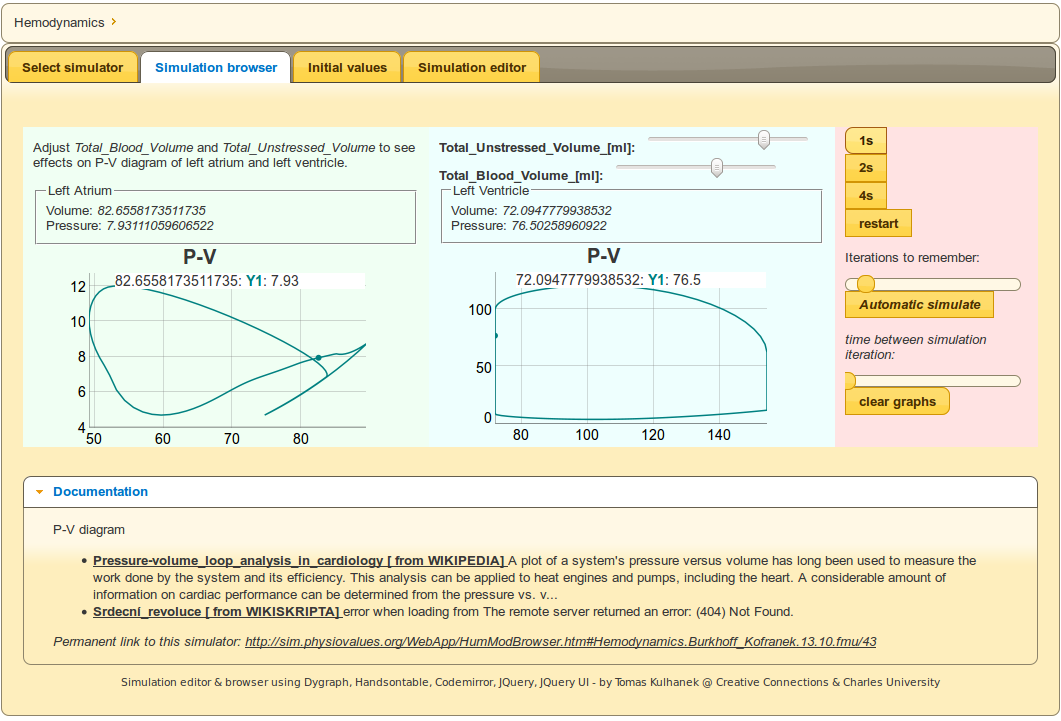
\includegraphics[width=1\textwidth]{chapter7/sim-physiovalues.png}
    \caption{Web application to visualize simulation. In this case pressure volume diagrams of left atrium and left ventricle of the model of hemodynamics of cardiovascular system.}
    \label{fig:sim.physiovalues}
\end{figure}

